\subsection{NN}

\subsubsection{Operation}
\begin{figure}[h]
	\centering
	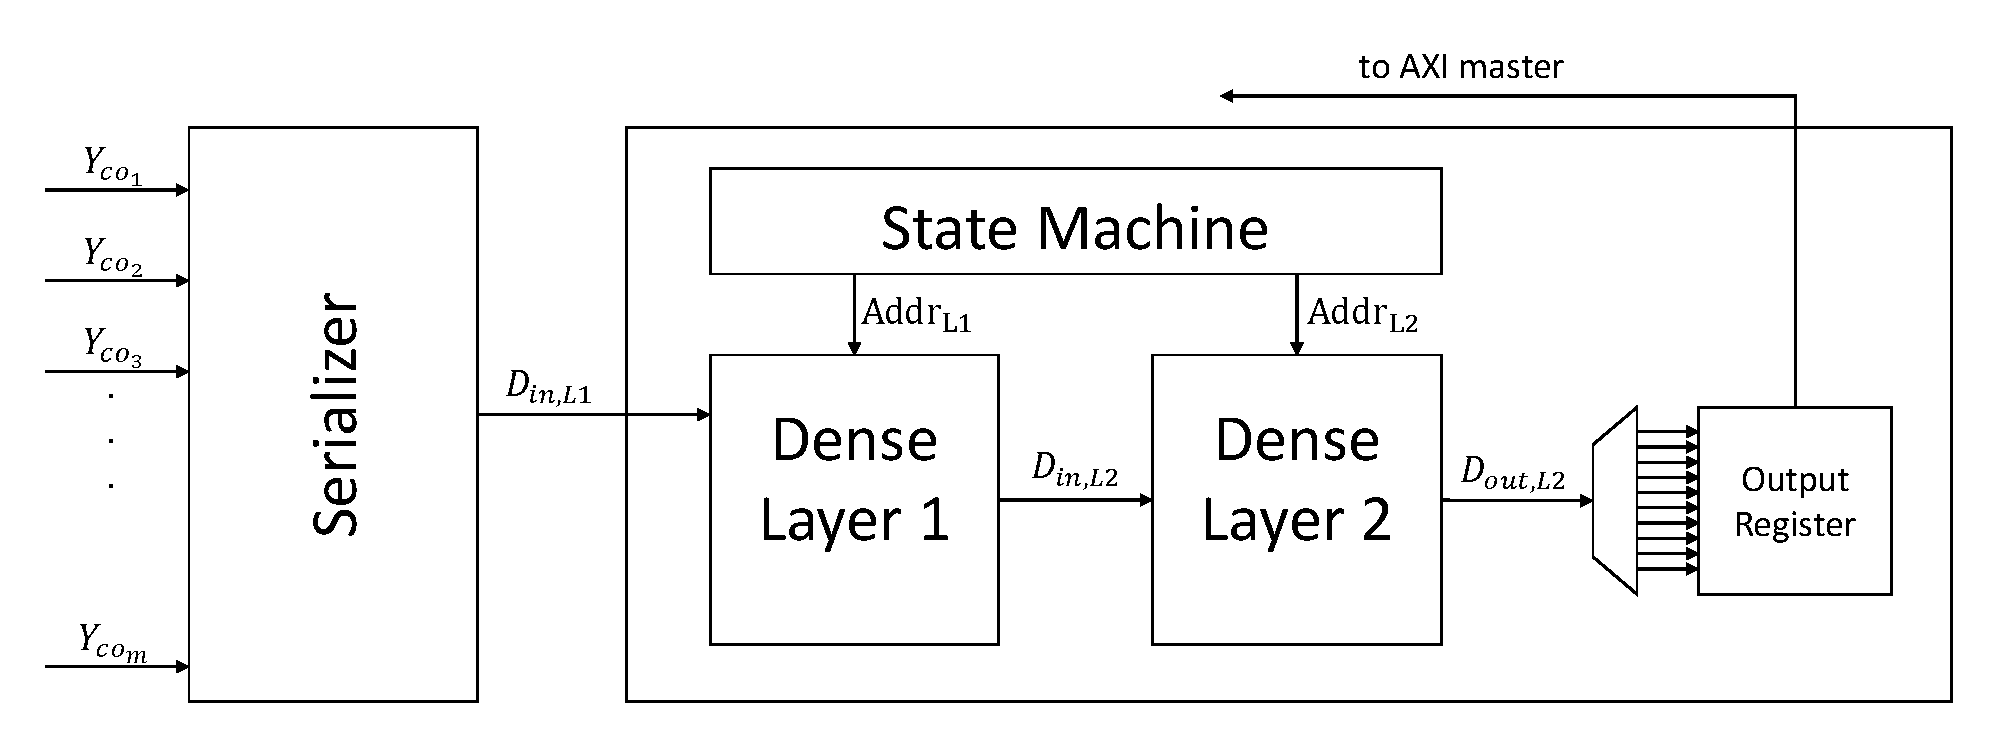
\includegraphics[width=1\textwidth]{img/dense.pdf}
	\caption{Diagram of the combined, fully connected NN.}
	\label{FIG:nn}
\end{figure}

The fully-connected neural network is shown in figure \ref{FIG:nn}. It consists of two dense layer instances controlled by a state machine. The output of layer 1 is fed directly into the layer 2. The output of layer 2 are 10 values which represent the confidence that the input image showed a specific number. 

The Serializer module is connected to the previous pooling layer. The $m=32$ output channels need to be converted into a stream of single values of length VECTOR\_WIDTH. For this, the previous pooling layer is stalled by keeping the ready signal low while a vector of $m$ values is serialized.

\subsubsection{Interface}
\begin{itemize}
	\item Input interface, a stream of values of length VECTOR\_WIDTH
	\item Output interface, a vector of 10 values of length VECTOR\_WIDTH
\end{itemize}
\subsubsection{Parameter}
\begin{itemize}
	\item VECTOR\_WIDTH: integer
	\item INPUT\_COUNT: integer
	\item OUTPUT\_COUNT: integer
\end{itemize}